\documentclass[10pt]{article}
\usepackage{amsmath,epsfig,amsthm,amssymb}
\usepackage{graphicx}
\usepackage{authblk}
\usepackage{mathrsfs}
\usepackage{amssymb}
\usepackage{hyperref}
\usepackage{ tipa }
\usepackage{listings}
\usepackage{enumitem}
\usepackage[svgnames]{xcolor}
\lstset{language=R,
    basicstyle=\small\ttfamily,
    stringstyle=\color{DarkGreen},
    otherkeywords={0,1,2,3,4,5,6,7,8,9},
    morekeywords={TRUE,FALSE},
    deletekeywords={data,frame,length,as,character},
    keywordstyle=\color{blue},
    commentstyle=\color{DarkGreen},
}


\setlength{\textheight}{9.2in} \setlength{\topmargin}{-1.0in}
\setlength{\textwidth}{440pt} \setlength{\oddsidemargin}{10pt}

\newcommand\Z{\mathbb Z}
\newcommand\R{\mathbb R}
\newcommand\Q{\mathbb Q}
\newcommand\N{\mathbb {N}}
\newcommand\cov{\textrm{Cov}}
\newcommand\E{\textrm{E}}
\newcommand\V{\textrm{Var}}
\newcommand\Span{\textrm{Span}}
\newcommand\Rref{\textrm{rref}}
\newcommand\vol{\textrm{vol}}
\title{15.458 Prject C: Portfolio and Risk Management}

\author{Ira Li, Mark Tang and Jingjie Zheng}

\date{\today}

\begin{document}
\maketitle

\begin{enumerate}
    \item[1.] \textbf{Beta:} Use the data from ``crispy04" to examine the CAPM beta between ``the market" and your favorite Dow stock for the period 1/1/2008 to 12/31/2009. Pick a stock that was in the DJIA for the entire period and then create and compare the following:
    \begin{enumerate}
        \item A time series plot of the 3-month rolling beta of the stock vs. the S\&P 500. (Use the stored, pre-computed values.) The primary tables to use are $\{$dailyvalue, benchvalue $\}$. Tables with supplementary attributes that may be useful include $\{$dim\textunderscore equity, bench, indexmember, and dim\textunderscore numtype$\}$.
        \begin{proof}[Answer] We picked Goldman Sachs as our favorite Dow stock. Below is the 3 month-rolling beta of the stock vs the S\&P 500,
        \begin{figure}[ht]
            \centering
            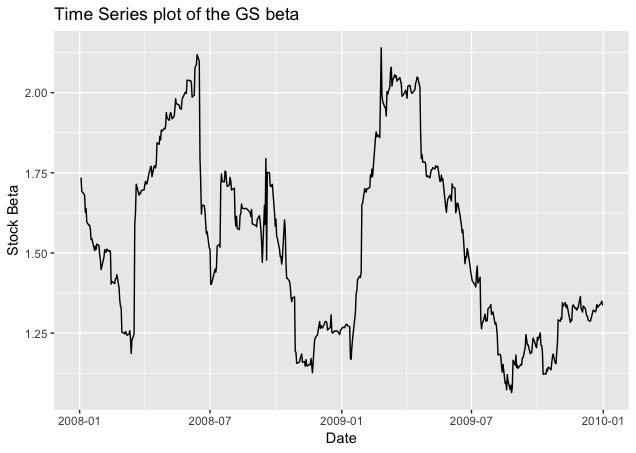
\includegraphics[scale = 0.45]{Q1a.jpeg}
            \caption{Times Series Plot of the GS Beta}
        \end{figure}
        \end{proof}
        
        
        
        
        \item A scatter plot of 1-day stock returns vs. the SPTR (S\&P 500 total return index) 1-day returns along with a line of best fit (OLS regression) and its slope equation. How does this result relate to, and compare with, the time series plot above?
        
        \begin{proof}[Answer] Below is the summary of OLS regression followed by the scatter plot. We see that the 1-day stock returns and the SPTR are positively correlated. 
        \begin{table}[ht]
\centering
\begin{tabular}{rrrrr}
  \hline
 & Estimate & Std. Error & t value & Pr($>$$|$t$|$) \\ 
  \hline
Intercept & 0.0002 & 0.0013 & 0.19 & 0.8525 \\ 
  Slope & 1.5052 & 0.0588 & 25.61 & 0.0000 \\ 
   \hline
\end{tabular}
\end{table}
        
        
        
        \begin{figure}[ht]
            \centering
            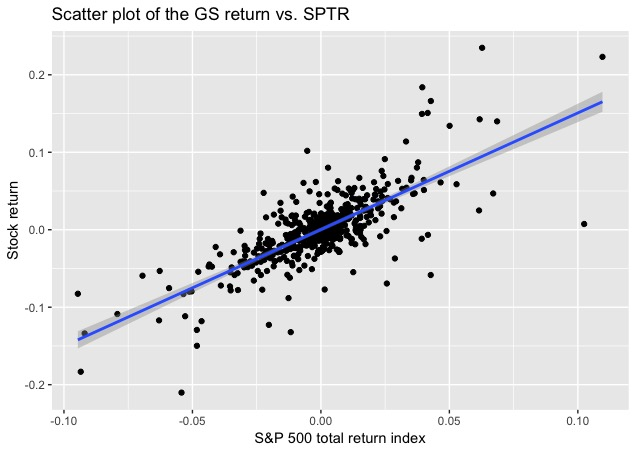
\includegraphics[scale = 0.45]{Q1b.jpeg}
            \caption{GS return vs. SPTR}
        \end{figure}

        
        
        
        \end{proof}
        
        \item A scatter plot of 1-day stock returns vs. the VIX (CBOE implied volatility index) 1-day returns along with regression line and its slope equation. Should the VIX be considered as a ``factor" in addition the ``the market" as part of a linear regression model for stock returns?
        \begin{proof}[Answer] Below is the summary of OLS regression followed by the scatter plot. We see that the 1-day stock returns and the VIX are negatively correlated. 
        
        \begin{figure}[ht]
            \centering
            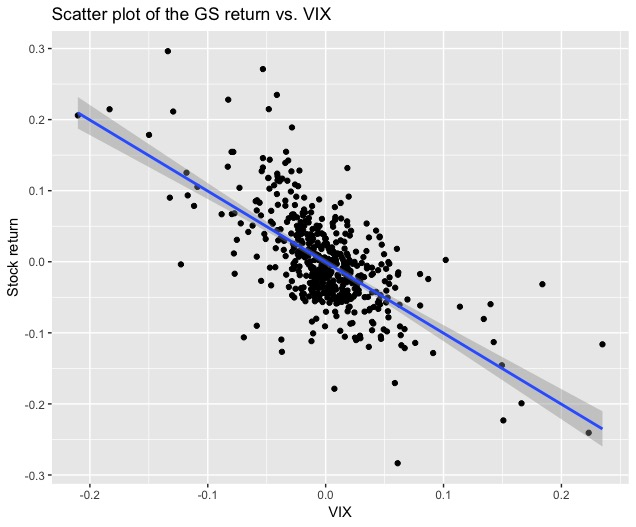
\includegraphics[scale = 0.45]{Q1c.jpeg}
            \caption{GS return vs. VIX}
        \end{figure}
        
        \begin{table}[h]
\centering
\begin{tabular}{rrrrr}
  \hline
 & Estimate & Std. Error & t value & Pr($>$$|$t$|$) \\ 
  \hline
Intercept & -0.0005 & 0.0023 & -0.22 & 0.8255 \\ 
 Slope & -0.9995 & 0.0527 & -18.96 & 0.0000 \\ 
   \hline
\end{tabular}
\end{table}

        \end{proof}
    \end{enumerate}
    
  
    \newpage
    
    \item[2.] \textbf{Performance modeling:} You are an evaluating a potential investment in a hedge fund. It is the end of 2004, and you have in-depth access to the fund’s daily position data for the period 2001-2004. Your goal is to characterize the past return profile in order to estimate its future success. Use the data for the equity long/short strategy called ``Contra01" in the OLAP database \textbf{StatArb03} using the cube \textbf{Positions03}. For performance results, use the weighted returns net of transaction costs, given by the fields ``Weighted Return Tc." Ignore hedge fund management fees.
    \begin{enumerate}
        \item  Give the annualized return, volatility, and Sharpe ratio (using $r_f=0$) for the strategy.
        \begin{proof}[Answer] Assume log returns and $r_f=0$, we summarize the statistics of the hedge fund performance as follows:
        \begin{table}[ht]
\centering
\begin{tabular}{ccc}
  \hline
  Annualized Return & Volatility & Sharpe Ratio \\ 
  \hline
  110.7\% & 24.5\% & 4.53 \\ 
   \hline
\end{tabular}
\end{table}
        
        \end{proof}
        \item  Use linear regression to report on the CAPM alpha, beta, and $R$-squared for the strategy, including standard errors of your estimates and $t$-statistics. Is the alpha statistically different from a CAPM prediction? How would you characterize the market-neutrality of the fund in light of its beta?
        \begin{proof}[Answer] Recall that the CAPM model suggests that 
        $$r-r_f = \alpha + \beta(r_M - r_f).$$
        Below is the summary for linear regression between hedge fund return and excess market return.
        \begin{table}[ht]
\centering
\begin{tabular}{rrrrr}
  \hline
 & Estimate & Std. Error & t value & Pr($>$$|$t$|$) \\ 
  \hline
$\alpha$ & 0.0043 & 0.0005 & 8.90 & 0.0000 \\ 
  $\beta$ & 0.0971 & 0.0402 & 2.42 & 0.0159 \\ 
   \hline
\end{tabular}

\medskip
\begin{tabular}{rrrr}
    \hline
     Observations  & Residual Std. Error  &  $R^2$     Adjusted & $R^2$ \\
     \hline
     1004      &       0.01536     &    0.005791   &   0.004799  \\
     \hline
\end{tabular}

\end{table}




        Notice that the P-value of $\alpha$ is close to zero, so the $\alpha$ is significantly different from CAPM prediction. Similarly, P-value of $\beta$ is less than 0.05, $\beta$ is significant, hence the hedge fund is not market-netural.
        \end{proof}
        
        \item Extend this regression model to include Fama-French factors, and repeat the analysis in the previous question. (Data is available in crispy04.dbo.famafrench.)
        \begin{proof}[Answer] Recall that the Fama-French model suggests that 
        $$r-r_f = \alpha + \beta_M(r_m -r_f) + \beta_{\textrm{SMB}}\cdot \textrm{SMB} + \beta_\textrm{{HML}}\cdot \textrm{HML} + \beta_\textrm{{UMD}}\cdot \textrm{UMD}$$
        Below is the summary for multi-linear regression between hedge fund return against the Fama-French factors.  Notice that $\alpha$ is significant since P-value of $\alpha$ is close to zero. All the beta's are insignificant as the P-value for every beta is greater than $0.05$. 
        
        \begin{table}[ht]
\centering
\begin{tabular}{rrrrr}
  \hline
 & Estimate & Std. Error & t value & Pr($>$$|$t$|$) \\ 
  \hline
$\alpha$ & 0.0044 & 0.0005 & 8.98 & 0.0000 \\ 
  $\beta_{M}$ & 0.0498 & 0.0511 & 0.97 & 0.3302 \\ 
   $\beta_{\textrm{SMB}}$ & -0.1514 & 0.0874 & -1.73 & 0.0837 \\ 
  $\beta_\textrm{{HML}}$ & 0.0483 & 0.1132 & 0.43 & 0.6700 \\ 
  $\beta_\textrm{{UMD}}$ & -0.1139 & 0.0661 & -1.72 & 0.0852 \\ 
   \hline
\end{tabular}

\medskip
\begin{tabular}{rrrr}
    \hline
     Observations  & Residual Std. Error  &  $R^2$     Adjusted & $R^2$ \\
     \hline
    1004        &     0.01533    &     0.01288      &0.00893      \\
     \hline
\end{tabular}


\end{table}

      

        \end{proof}
        \newpage 
        \item Plot the strategy one-day returns in order, from lowest to highest. What fraction of days were winners and what fraction were losers? What was the median return of winners and what was the median return of the losers?
        \begin{proof}[Answer] See below
        \begin{figure}[ht]
            \centering
            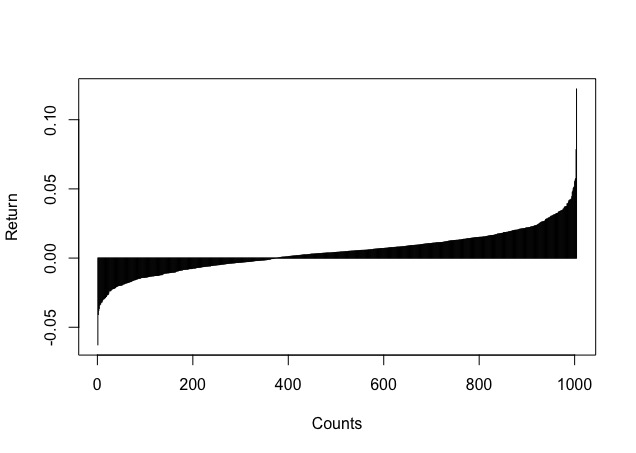
\includegraphics[scale = 0.5]{Q2d.jpeg}
            \caption{Strategy one-day ordered return}
            \label{fig:my_label}
        \end{figure}
        
        
        \begin{table}[ht]
\centering
\begin{tabular}{ccc}
  \hline
 & Winners & Losers \\ 
  \hline
Fracation & 63.75\% & 37.25\% \\ 
  Median & 1.02\% & -0.80\% \\ 
   \hline
\end{tabular}
\end{table}
        
        
        
        \end{proof}
        
        
        \item Based on your analysis in 2004, how do you expect the fund to perform for the five-year period ahead?
        \begin{proof}[Answer] Based on the Fama-French model, we see that the fund is netural to all Fama-French factors and has a significant alpha. Thus, we would expect the fund to perform very well in the upcoming five-year period.
        
        \end{proof}
    \end{enumerate}
  




    \item[3.] \textbf{Performance attribution:} Analyze the performance of the contrarian equity long/short strategy ``Contra01" over the period 2005-2009 using the data in the OLAP database \textbf{StatArb03} using the cube \textbf{Positions03}. For performance results, use the weighted returns net of transaction costs, given by the fields ``Weighted Return Tc"
    \begin{enumerate}
        \item  Give the annualized return, volatility, and Sharpe ratio (using $r_f=0$) for the strategy overall and for the long and short halves of the strategy. (That is, do the same calculations just using the long positions and then just the short positions.)
        \begin{proof}[Answer] Assume log returns and $r_f=0$, we summarize the statistics of the hedge fund's long strat, short strat and combined weigted returns as follows:
        \begin{table}[ht]
\centering
\begin{tabular}{rrrr}
  \hline
 & Annualized Return & Volatility & Sharpe Ratio \\ 
  \hline
Long & -0.21 & 0.32 & -0.65 \\ 
  Short & 0.58 & 0.29 & 2.03 \\ 
  Combined & 0.37 & 0.28 & 1.31 \\ 
   \hline
\end{tabular}
\end{table}
        
        
        
        \end{proof}
        
        \item Use linear regression to report on the CAPM alpha, beta, and $R$-squared for the strategy, including standard errors of your estimates and t-statistics. Is the alpha statistically different from a CAPM prediction? How would you characterize the market-neutrality of the fund in light of its beta?
        \begin{proof}[Answer] Below is the summary for linear regression result. We see that the $\alpha$ is significant, $\beta$ is not significant hence the hedge fund is market neutral. 
        \begin{table}[ht]
\centering
\begin{tabular}{rrrrrr}
  \hline
 & Estimate & Std. Error & t value & Pr($>$$|$t$|$)\\ 
  \hline
$\alpha$ & 0.0014 & 0.0005 & 2.70 & 0.0071 \\ 
  $\beta$ & 0.0105 & 0.0332 & 0.32 & 0.7512 \\
   \hline
\end{tabular}

\medskip
\begin{tabular}{rrrr}
    \hline
     Observations  & Residual Std. Error  &  $R^2$     Adjusted & $R^2$ \\
     \hline
    1004        &     0.01533    &     0.01288      &0.00893      \\
     \hline
\end{tabular}
\end{table} 
 

        
    
        \end{proof}        
        
        
        \item Plot the strategy one-day returns in order, from lowest to highest. What fraction of days were winners and what fraction were losers? What was the median return of winners and what was the median return of the losers?
        \begin{proof}[Answer] See next page for the summary of winners and losers.
        
        \begin{figure}[h]
            \centering
            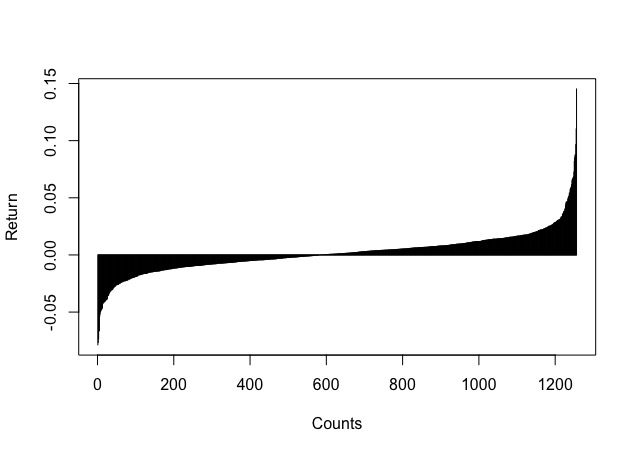
\includegraphics[scale = 0.4]{Q3c.jpeg}
            \caption{Strategy one-day ordered return}
        \end{figure}
    
       \begin{table}[ht]
\centering
\begin{tabular}{rrr}
  \hline
 & Winners & Losers \\ 
  \hline
Fracation & 53.5\% & 46.5\%\\ 
  Median & 0.83\% & -0.82\% \\ 
   \hline
\end{tabular}
\end{table}
        
       

                
        
        
        \end{proof}   
        
        \newpage 
        \item How do these results compare with your predictions from the period 2001-2004 from Question \#2 above? Do you believe the portfolio manager's style changed or remained constant over time? Why or why not?
        \begin{proof}[Answer] Comparing the manager's performance from 2001-2004 to his performance from 2005-2009, based on CAMP regression, we conclude that the manager is not market neutral from 2001-2004 but market neutral from 2005-2009. Further, the change of winners and losers break down of these two periods corroborate the change of investment style. 
        
        
        
        \end{proof}          
        
        
        \item Which SIC sector contributed the largest total return, in absolute value, for calendar year 2006? What was the return, and what fraction of strategy total return did it contribute? (A plot or table of total weighted return, aggregated by sector and filtered on 2006 tradedates would be helpful.)
        \begin{proof}[Answer] We performed the analysis using Excel with a query table linked to the OLAP database \textbf{StatArb03} using the cube \textbf{Positions03}. We filtered with ``Domain = Contra01'' and ``Time = Calendar 2006'', presented in the following table:
        
\begin{table}[ht]
\centering
\begin{tabular}{lrrr}
  \hline
  SIC Sectors & \begin{tabular}{@{}c@{}} Weighted Return \\Tc Abs \end{tabular} & \begin{tabular}{@{}c@{}} Weighted Return \\Tc \end{tabular} & \begin{tabular}{@{}c@{}} Fraction of Strategy \\ Total Return \end{tabular} \\ 
  \hline
  \begin{tabular}{@{}c@{}} Agriculture Forestry, \\ and Fishing\end{tabular} & 0.028 & 0.003 & 0.6\% \\ 
  Construction & 0.101 & -0.005 & -1.1\% \\ 
  Finance, Insurance, and Real Estate & 0.969 & 0.093 & 21.3\% \\ 
  Manufacturing & 8.018 & 0.212 & 48.2\% \\ 
  Mining & 0.537 & 0.063 & 14.3\% \\ 
  Retail Trade & 0.667 & -0.011 & -2.6\% \\ 
  Services & 3.813 & 0.056 & 12.8\% \\ 
  \begin{tabular}{@{}c@{}} Transportation, Communications, \\Electric, Gas, and Sanitary Services\end{tabular} & 1.123 & 0.008 & 1.8\% \\ 
  Wholesale Trade & 0.919 & 0.020 & 4.7\% \\
  \hline
  Grand Total & 16.175 & 0.439 & 100.0\% \\ 
   \hline
\end{tabular}
\end{table}
        
        The manufacturing sector contributed the largest total return in 2006 in absolute value, with return of 21.2\%, or 8.018 in absolute value, accounting for 48.2\% of strategy total return.
        
        \end{proof}         
        
        \newpage
        
        \item Same as previous question using GICS sectors.
        \begin{proof}[Answer] Again, using Excel query with filters, ``Domain = Contra01'' and ``Time = Calendar 2006'', we derive the following table:
        
\begin{table}[ht]
\centering
\begin{tabular}{lrrr}
  \hline
GICS Sectors & \begin{tabular}{@{}c@{}} Weighted Return \\Tc Abs \end{tabular} & \begin{tabular}{@{}c@{}} Weighted Return \\Tc \end{tabular} & \begin{tabular}{@{}c@{}} Fraction of Strategy \\ Total Return \end{tabular} \\ 
  \hline
  NA & 7.219 & 0.194 & 44.3\% \\ 
  Energy & 0.515 & 0.042 & 9.5\% \\ 
  Materials & 0.310 & -0.013 & -3.0\% \\ 
  Industrials & 1.121 & 0.079 & 18.1\% \\ 
  Consumer Discretionary & 1.191 & 0.006 & 1.4\% \\ 
  Consumer Staples & 0.382 & 0.017 & 3.9\% \\ 
  Health Care & 2.098 & -0.002 & -0.4\% \\ 
  Financials & 0.564 & 0.058 & 13.3\% \\ 
  Information Technology & 2.667 & 0.059 & 13.5\% \\ 
  Telecommunication Services & 0.074 & -0.014 & -3.1\% \\ 
  Utilities & 0.033 & 0.011 & 2.5\% \\ 
  \hline
  Grand Total & 16.175 & 0.439 & 100.0\% \\ 
   \hline
\end{tabular}
\end{table}
        
        The sector ``NA'' (meaning stocks that have no specific GICS sector classification) contributed the largest total return in 2006 in absolute value, with return of 19.4\%, or 7.219 in absolute value, accounting for 44.3\% of strategy total return.
        
        \medskip
        If we consider ``NA'' not as a sector and exclude it from analysis, then the Information Technology sector  contributed the largest total return in 2006 in absolute value, with return of 5.9\%, or 2.667 in absolute value, accounting for 13.5\% of strategy total return.
        
        \end{proof}   
        
        
    \end{enumerate}
    
    \item[4.] \textbf{Risk measurement:} Analyze the exposures of the contrarian equity long/short strategy ``Contra01'' using the fund data for 2005-2009 in the OLAP database \textbf{StatArb03} using the cube \textbf{Positions03}. This strategy focused on security selection and mean-reversion dynamics at the individual stock level. While the overall longs and shorts were constrained to be balanced, the individual sectors and other factors were not. Use the data on the history of portfolio exposures, measured primarily by aggregating security weights, to answer the following.
    \begin{enumerate}
        \item For each GICS sector, give its highest and lowest net exposure over the period 2005-2009. Which sectors stayed within +/- 10\% of portfolio weight throughout?
        \begin{proof}[Answer] Using the Excel linked query table with filters ``Domain = Contra01'' and ``Time = Calendar 2005-2009'', we obtained the daily exposure for each GICS sector. A simple analysis in Excel shows:
        
\begin{table}[ht]
\centering
\begin{tabular}{lrr}
  \hline
  GICS Sectors & Maximum Weight & Minimum Weight \\ 
  \hline
  NA & 0.310 & -0.222 \\ 
  Energy & 0.310 & -0.233 \\ 
  Materials & 0.169 & -0.127 \\ 
  Industrials & 0.163 & -0.190 \\ 
  Consumer Discretionary & 0.194 & -0.240 \\ 
  Consumer Staples & 0.092 & -0.080 \\ 
  Health Care & 0.241 & -0.222 \\ 
  Financials & 0.333 & -0.487 \\ 
  Information Technology & 0.241 & -0.236 \\ 
  Telecommunication Services & 0.042 & -0.051 \\ 
  Utilities & 0.035 & -0.048 \\ 
  \hline
  Grand Total & 0.030 & -0.054 \\ 
   \hline
\end{tabular}
\end{table}
        
        The Consumer Staples Sector, the Telecommunication Service Sector, and the Utilities Sector stayed within +/- 10\% of portfolio weight throughout.
        
        \end{proof}
        
        \item On 9/15/2008, which GICS sector was the most unbalanced? Give the total portfolio weight long, total weight short, and net portfolio weight for that sector. What was the day's portfolio return?
        \begin{proof}[Answer] Using the Excel linked query table with filters ``Domain = Contra01'' and ``Date = 09/15/2008'', we obtain:
        
\begin{table}[ht]
\centering
\begin{tabular}{lrrr}
  \hline
  GICS Sectors & Total Weight Long & Total Weight Short & Net Portfolio Weight \\ 
  \hline
  NA & 0.366 & -0.254 & 0.113 \\ 
  Energy & 0.014 & -0.085 & -0.070 \\ 
  Materials & 0.014 & -0.014 & 0.000 \\ 
  Industrials & 0.056 & -0.085 & -0.028 \\ 
  Consumer Discretionary & 0.099 & -0.183 & -0.085 \\ 
  Consumer Staples & 0.000 & -0.014 & -0.014 \\ 
  Health Care & 0.211 & -0.141 & 0.070 \\ 
  Financials & 0.085 & -0.113 & -0.028 \\ 
  Information Technology & 0.155 & -0.099 & 0.056 \\ 
  \hline
  Grand Total & 1.000 & -0.986 & 0.014 \\ 
   \hline
\end{tabular}
\end{table}
        
        On 09/15/2008, the ``NA'' sector was the most unbalanced. Its total portfolio weight long was 36.6\%, total portfolio weight short was -25.4\%, and net portfolio weight was 11.3\%.
        
        \medskip
        If we consider ``NA'' not as a sector and exclude it from analysis, then the Consumer Discretionary sector was the most unbalanced. Its total portfolio weight long was 9.9\%, total portfolio weight short was -18.3\%, and net portfolio weight was -8.5\%.
        
        \medskip
        That day's portfolio return was -4.65\% (before transaction costs) and -4.80\% (after transaction costs).
        
        \end{proof} 
        


        \item Same as previous question for 2/27/2007.
        \begin{proof}[Answer] Using the Excel linked query table with filters ``Domain = Contra01'' and ``Date = 02/27/2007'', we obtain:
        
\begin{table}[ht]
\centering
\begin{tabular}{lrrr}
  \hline
 GICS Sectors & Total Weight Long & Total Weight Short & Net Portfolio Weight \\ 
  \hline
  NA & 0.341 & -0.280 & 0.061 \\ 
  Energy & 0.012 & -0.024 & -0.012 \\ 
  Materials & 0.037 & -0.037 & 0.000 \\ 
  Industrials & 0.110 & -0.061 & 0.049 \\ 
  Consumer Discretionary & 0.110 & -0.098 & 0.012 \\ 
  Consumer Staples & 0.037 & -0.012 & 0.024 \\ 
  Health Care & 0.122 & -0.122 & 0.000 \\ 
  Financials & 0.073 & -0.061 & 0.012 \\ 
  Information Technology & 0.134 & -0.280 & -0.146 \\ 
  Telecommunication Services & 0.024 & -0.012 & 0.012 \\ 
  \hline
  Grand Total & 1.000 & -0.988 & 0.012 \\ 
   \hline
\end{tabular}
\end{table}
        
        On 07/27/2007, the Information Technology sector was the most unbalanced. Its total portfolio weight long was 13.4\%, total portfolio weight short was -28.0\%, and net portfolio weight was -14.6\%.
        
        \medskip
        That day's portfolio return was 0.59\% (before transaction costs) and 0.44\% (after transaction costs).
        
        \end{proof}

        
        
        \item Suppose a sub-strategy were defined by restricting the ``Contra01'' portfolio weights and returns to the GICS Financials sector only. Is this sub-strategy ``market-neutral'' on its own? How do the sub-strategy exposures evolve over time in the absence of constraints? Plot and the net long/short exposure as well as the gross long vs. gross short exposures. 
        \begin{proof}[Answer] Using Excel linked query table, we extracted time-series data of weighted return (before transaction costs) of this sub-strategy. We then run a regression on this time series against market return in 2005-2009, applying the CAPM model. Regression result as below: 
        
\begin{table}[ht]
\centering
\begin{tabular}{rrrrrr}
  \hline
 & Estimate & Std. Error & t value & Pr($>$$|$t$|$)\\ 
  \hline
$\alpha$ & 0.0003044 & 0.0001737 & 1.753 & 0.0799 \\ 
  $\beta$ & -0.0035573 & 0.0114361 & -0.311 & 0.7558 \\
   \hline
\end{tabular}

\medskip
\begin{tabular}{rrrr}
    \hline
     Observations  & Residual Std. Error  &  $R^2$     Adjusted & $R^2$ \\
     \hline
    1259        &     0.006162    &     0.00007697      & -0.0007185      \\
     \hline
\end{tabular}
\end{table} 
        
        The beta estimate has a t-stat of -0.311, which is insignificant at the 5\% significance level, and we fail to reject the null hypothesis that beta is zero. With a zero beta, the sub-strategy can be considered as ``market-neutral'' on its own.
        
        \medskip
        Besides, a time-series plot of the sub-strategy exposure is shown below.
        
        \begin{figure}[ht]
            \centering
            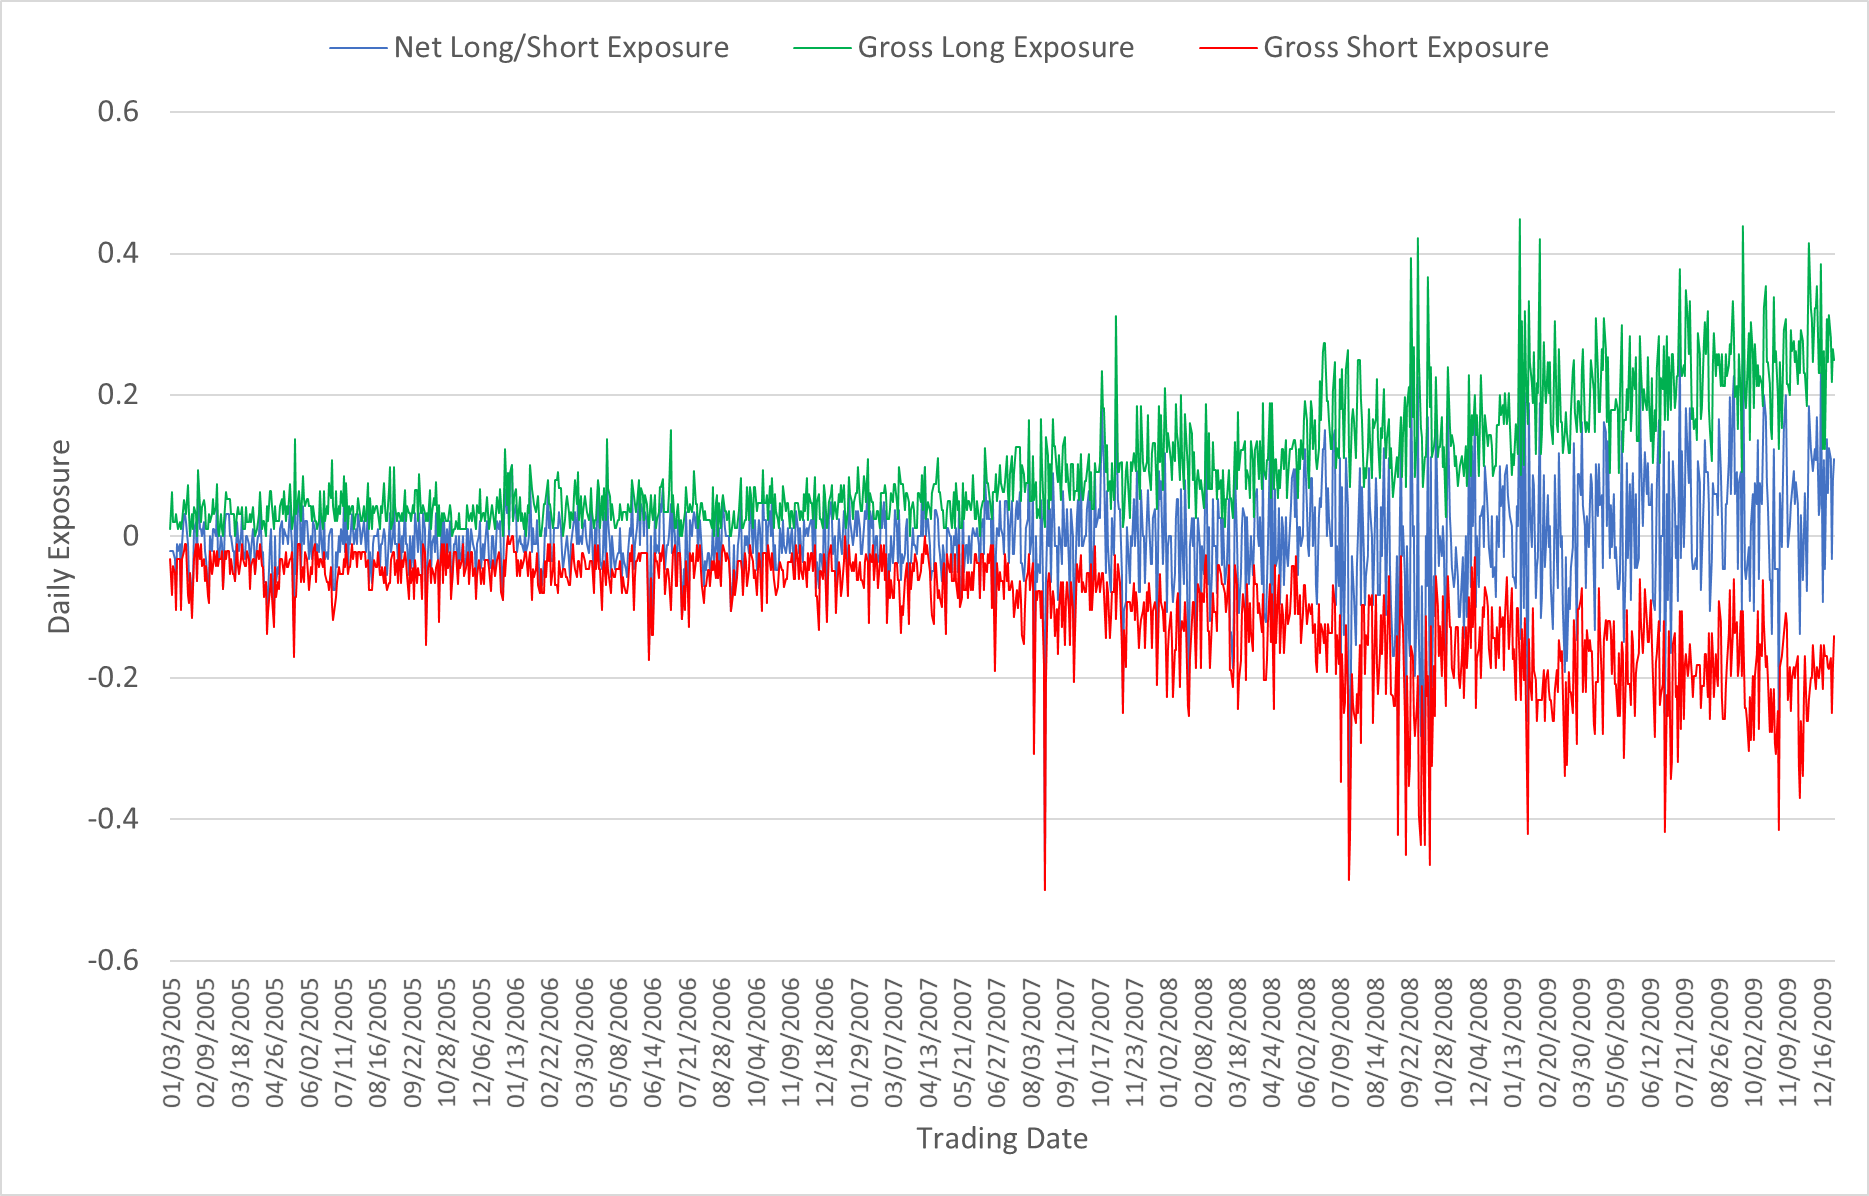
\includegraphics[scale = 0.7]{Q4d2.png}
            \caption{Daily Exposure of Financial-Sector-Only Sub-Strategy}
        \end{figure}
        
        
        
        
        
        As seen from the plot, the exposure in absolute value stayed low before mid-2007 and started increasing steadily since then.
        
        \end{proof}
    \end{enumerate}


    \item[5.] \textbf{Correlation dynamics:} Analyze the behavior of the \textit{average correlation} among stocks in the Dow Jones Industrial Average for the period 2008-2009 using the data in \textbf{crispy04}. Create two plots: one for a 1-month correlation window and the second using a 3-month window. On each graph, plot lines for the following daily time series:
    \begin{enumerate}
        \item Average (``implied'') correlation, as discussed in class,
        $$ \overline{\rho} \equiv \dfrac{\sigma_p^2 - \sum_{i=1}^N w_i^2\sigma_i^2}{2\sum_{i<j} w_iw_j \sigma_i\sigma_j} = \dfrac{\sigma_p^2 - \sigma_{(0)}^2}{\sigma_{(1)}^2 - \sigma_{(0)}^2}$$
    
        
        \item Index realized variance 
        \item $\textrm{Index variance}_0$, the variance the index would have if all member correlations were zero.
              
        \item $\textrm{Index variance}_1$, the variance the index would have if all member correlations were 100\%.
        \smallskip
        \textbf{Data Cleaning}:  We gained raw data from Crispy04 for both index and 35 individual components that was at least once consisted in DJIA index during the period 2008 - 2009. Then, by adjusting the portfolio to correspond to the three rebalancing attempts for DJIA composition, we got the proper data for further analysis. 
        
        \smallskip
        \textbf{Data Processing and Computing}:
        we then assigned the weights for each individual stock everyday and calculate the index realized variance, index variance if all member correlation were zero, and index variance if all member correlation were one. Lastly, we computed the implied volatility via the formula. 
        
        \begin{figure}[htbp]
            \centering
            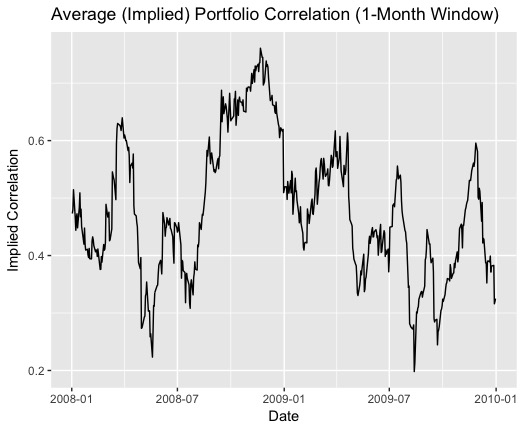
\includegraphics[scale = 0.7]{Q5_rho_1m.jpeg}
            \caption{Times Series Plot of Average correlation (1-month Window)}
        \end{figure}
        
        \begin{figure}[htbp]
            \centering
            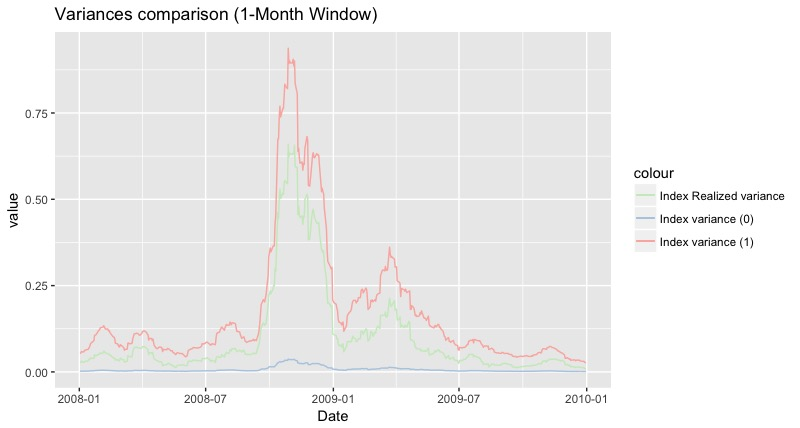
\includegraphics[scale = 0.5]{Q5_var_1m.jpeg}
            \caption{Times Series Plot of Variances under different assumptions (1-month Window)}
        \end{figure}
        
        \begin{figure}[htbp]
            \centering
            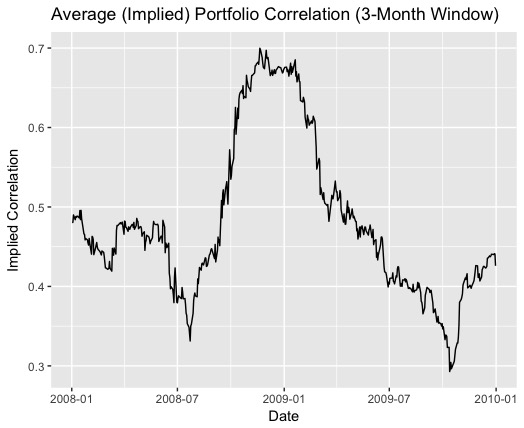
\includegraphics[scale = 0.7]{Q5_Rho_3m.jpeg}
            \caption{Times Series Plot of Average correlation (3-month Window)}
        \end{figure}
        
        \begin{figure}[htbp]
            \centering
            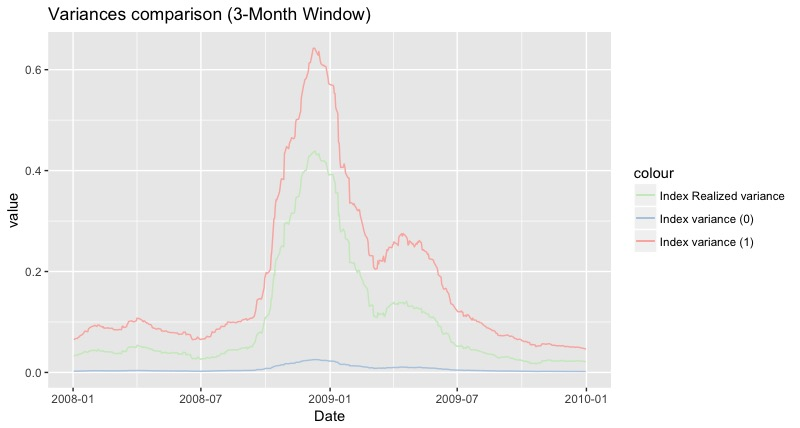
\includegraphics[scale = 0.5]{Q5_var_3m.jpeg}
            \caption{Times Series Plot of Variances under different assumptions (3-month Window)}
        \end{figure}
        
        
        
        
        \newpage
        \item For each window size, what is the maximum value of the average correlation and when does it occur?
        \begin{proof}[Answer]
        
        The maximum correlation is 0.76 under 1-month window size and 0.70 under 3-month window size. Maximum correlation happens at 2008-11-21 under 1-month window size and 2008-11-20 under 3-month window size. As we can see in the graphs for both window size, implied volatility tends to increase as the variance of index increases. Also, because 3-month correlation incorporates more past movements, as a result, the time series is more smooth compared to 1-month window size where everything is more noisy. However, even though the 3-month model may react to big changes a little slower, both time horizon models generate similar results and show similar relationship with the variances. 
        
   
        \end{proof}        
        
        
        \item What constraints should be satisfied by the four values? Do they hold for the period in question?
        \begin{proof}[Answer]
        First of all, implied correlation should be in the range between -1 and 1 to be meaningful. Secondly, value of $\textrm{Index variance}_0$ should always be lower than the value of $\textrm{Index variance}_1$ because $\textrm{Index variance}_1$ takes positive covariance terms into account. Lastly, the realized variance should be lower than $\textrm{Index variance}_1$ and higher than \\$\textrm{Index variance}_0$ since the implied correlation stays positive over the period. All of the constraints hold for the period 2008-2009.
        
        \end{proof}        
        
        \item What could cause the constraints to be violated?
        \begin{proof}[Answer]
        
        Because the implied correlation is calculated by using correct formula that fits in every situation, correlation will always stays in the range as long as the variances are in their proper range. However, if the variances data fails to make sense, for example, if variance happens to be smaller than 0, then everything else may consequently break the constraint.  
        
        \end{proof}        
    
    \end{enumerate}
    



    

    
    

\end{enumerate}


\newpage
\section*{Appendix}
\subsubsection*{Q1 R code}
\begin{lstlisting}[language=R]
library('csv')
library('dplyr')
library('readxl')
library('aTSA')
library('outliers')
library('quantmod')
library('ggplot2')
library('xtable')

setwd("~/Desktop/15.458 Financial Data Science/PS3")
dt <- read.csv("problem1.csv",header=TRUE)
colnames(dt) = c('Date','SPX','SPTR','VIX','GS','beta')
dt$Date = as.Date(dt$Date,"%Y/%m/%d")

#check data integrity
sum(is.na(dt$GS))
sum(is.na(dt$SPX))
sum(is.na(dt$SPTR))
sum(is.na(dt$VIX))
sum(is.na(dt$beta))

#---------------------------------------------------------------------------------------#

#1a) Time series of beta vs. SPX
scatterplot_a = ggplot(dt, aes(x=Date, y=beta)) + geom_line()
scatterplot_a  = scatterplot_a  +labs(x = "Date",y='Stock Beta', title='Time Series plot of the GS beta')
scatterplot_a

#---------------------------------------------------------------------------------------#

#1b)scatter plot of GS return vs. SPTR
scatterplot_b = ggplot(dt, aes(x=SPTR, y=GS)) + geom_point()
scatterplot_b = scatterplot_b  +labs(x = "S&P 500 total return index",y='Stock return', title='Scatter plot of the GS return vs. SPTR')
scatterplot_b 
# Add the regression line
scatterplot_b + geom_smooth(method=lm)

#linear regression equation
ols_b = lm(dt$GS ~ dt$SPTR)
summary(ols_b)

#---------------------------------------------------------------------------------------#

#1c)scatter plot of GS return vs. VIX
scatterplot_c = ggplot(dt, aes(x=GS, y=VIX)) + geom_point()
scatterplot_c  = scatterplot_c  +labs(x = "VIX",y='Stock return', title='Scatter plot of the GS return vs. VIX')
scatterplot_c 
# Add the regression line
scatterplot_c + geom_smooth(method=lm)

#linear regression equation
ols_c = lm(dt$VIX ~ dt$GS)
summary(ols_c)


\end{lstlisting}


\subsubsection*{Q2 R code}
\begin{lstlisting}
library('csv')
library('dplyr')
library('readxl')
library('aTSA')
library('outliers')
library('quantmod')
library('ggplot2')
library('scales')
library('xtable')

setwd("~/Desktop/15.458 Financial Data Science/PS3")
dt <- read.csv("Q2return.csv",header=TRUE)
colnames(dt) = c('Date','Return')
dt$Date = as.Date(dt$Date,"%m/%d/%Y")
df.fama = read.table("Q2FamaFrench(01-04).txt", sep = ',', header = TRUE)
colnames(df.fama) = c('Date','Risk Free Rate', 'Market Excess Return',
                      'SMB', 'HML', 'UMD')
df.fama$Date = as.Date(df.fama$Date,"%Y/%m/%d")

#---------------------------------------------------------------------------------------#
#1a) annualized return, volatility and SR, assume log return

ann_return = mean(dt$Return)*252
vol =  sqrt(252)*sd(dt$Return)
sr = ann_return/vol
df.a = data.frame(ann_return,vol,sr)
colnames(df.a) = c('Annualized Return', 'Volatility', 'Sharpe Ratio')

#2b) CAPM

answer2b = summary(lm((dt$`Return`-df.fama$`Risk Free Rate`)~df.fama$`Market Excess Return`)
)

#2c) 

answer2c = summary(lm((dt$`Return`-df.fama$`Risk Free Rate`)~df.fama$`Market Excess Return`+df.fama$SMB + df.fama$HML + df.fama$UMD)
)

#2d)

plot(sort(dt$Return), type = 'h',ylab = 'Return', xlab = 'Counts')

frac_winners =  length(which(dt$Return>0))/length(dt$Return)
frac_losers = length(which(dt$Return<0))/length(dt$Return)
median_winners = median( dt$Return[which(dt$Return>0)])
median_losers = median( dt$Return[which(dt$Return<0)])
df.d = data.frame(c(frac_winners,median_winners),c(frac_losers,median_losers))
colnames(df.d) = c('Winners', 'Losers')
rownames(df.d) = c('Fracation', 'Median')


\end{lstlisting}



\subsubsection*{Q3 R code}
\begin{lstlisting}

library('csv')
library('dplyr')
library('readxl')
library('aTSA')
library('outliers')
library('quantmod')
library('ggplot2')
library('scales')
library('xtable')

setwd("~/Desktop/15.458 Financial Data Science/PS3")
dt <- read.csv("Q3return.csv",header=TRUE)
colnames(dt) = c('Date','Long','Short','Combined')
dt$Date = as.Date(dt$Date,"%m/%d/%Y")
df.fama = read.table("Q3FamaFrench(05-09).txt", sep = ',', header = TRUE)
colnames(df.fama) = c('Date','Risk Free Rate', 'Market Excess Return',
                       'SMB', 'HML', 'UMD')
df.fama$Date = as.Date(df.fama$Date,"%Y-%m-%d")

#---------------------------------------------------------------------------------------#
#1a) annualized return, volatility and SR, assume log return for long-short strategy
 
f <- function(x){
  ann_return = mean(x)*252
  vol =  sqrt(252)*sd(x)
  sr = ann_return/vol
  c(ann_return,vol,sr)
}

df.a = apply(dt[,-1],2,f)
rownames(df.a) = c('Annualized Return', 'Volatility', 'Sharpe Ratio')

#2b) CAPM
df = df= merge(dt,df.fama, by = "Date")
answer2b = summary(lm((df$`Combined`-df$`Risk Free Rate`)~df$`Market Excess Return`))


#2d)
plot(sort(dt$Combined), type = 'h',ylab = 'Return', xlab = 'Counts')

frac_winners =  length(which(dt$Combined>0))/length(dt$Combined)
frac_losers = length(which(dt$Combined<0))/length(dt$Combined)
median_winners = median( dt$Combined[which(dt$Combined>0)])
median_losers = median( dt$Combined[which(dt$Combined<0)])
df.d = data.frame(c(frac_winners,median_winners),c(frac_losers,median_losers))
colnames(df.d) = c('Winners', 'Losers')
rownames(df.d) = c('Fracation', 'Median')



\end{lstlisting}


\subsubsection*{Q4 R code}
\begin{lstlisting}
#import data regression
dt4_e_r <- read.csv("Q4d1 - Contra01-GICSfinancial-Weights&Returns.csv",header=TRUE)
dt4_e_mkt <- read_csv("~/Desktop/MIT/Fall 2018/Data Science/Project C/Q3 - FamaFrench (05-09).txt")
#clean the data
dt4_e_mkt$d = as.Date(dt4_e_mkt$d,"%Y-%m-%d")
dt4_e_r$Trade.Date = as.Date(dt4_e_r$Trade.Date,"%m/%d/%Y")

ols4_e = lm((dt4_e_r$Weighted.Return-dt4_e_mkt$rf_str) ~ (dt4_e_mkt$mkt_str-dt4_e_mkt$rf_str))
summary(ols4_e)


\end{lstlisting}


\subsubsection*{Q5 R code}
\begin{lstlisting}
#---------------------------------------------------------------------------------------#
#5 correlation
#---------------------------------------------------------------------------------------#
#import the data
dt5_comp <- read.csv("~/Desktop/MIT/Fall 2018/Data Science/Project C/Q5 query - Comp Stocks.csv",header=TRUE)
dt5_djia <- read.csv("~/Desktop/MIT/Fall 2018/Data Science/Project C/Q5 query - DJIA.csv",header=TRUE)
dt5_comp = as.data.frame(dt5_comp)
dt5_comp$d = as.Date(dt5_comp$d,"%Y-%m-%d")
dt5_comp = dt5_comp[order(dt5_comp$d),]

#check integrity (505 days in total)
test_group = group_by(dt5_comp,ticker)
test_statistis = summarise(test_group,
                           count = n()
)

#---------------------------------------------------------------------------------------#
#clean the data to match djia composition
row_to_keep = which((dt5_comp$d < 2018-02-18 & !(dt5_comp$ticker %in% c('BAC','CVX','KFT','CSCO','TRV'))) | 
                      (dt5_comp$d > 2018-02-18 & dt5_comp$d < 2018-09-22 & !(dt5_comp$ticker %in% c('MO','HON','KFT','CSCO','TRV'))) |
                      (dt5_comp$d > 2018-09-22 & dt5_comp$d < 2019-06-08 & !(dt5_comp$ticker %in% c('MO','HON','AIG','CSCO','TRV'))) |
                      (dt5_comp$d > 2019-06-08 & !(dt5_comp$ticker %in% c('MO','HON','AIG','C','GM')))
)

dt5_comp = dt5_comp[row_to_keep,]

grouped_data <- group_by(dt5_comp,d)
statistics <- summarise(grouped_data,
                        count = n(),
                        total_p = sum(price)#,
                        #weight_sum = sum(weight)
) 
statistics = as.data.frame(statistics)

dt5_comp$weight = NA

#---------------------------------------------------------------------------------------#
#assign weight
for (i in 1:nrow(dt5_comp)) {
  for (j in 1:30) {
    dt5_comp$weight[i] = dt5_comp$price[i] / statistics$total_p[ceiling(i/30)]
  }
}

#---------------------------------------------------------------------------------------#
#calculate index variance (sigma_p^2)
DJIA_one_month = dt5_djia[dt5_djia$nm_numtype == 'vol_021',]
DJIA_three_month = dt5_djia[dt5_djia$nm_numtype == 'vol_063',]

DJIA_one_month$index_variance = DJIA_one_month$value^2
DJIA_three_month$index_variance = DJIA_three_month$value^2

#clean DJIA data
df_DJIA_1m = as.data.frame(DJIA_one_month)%>%
  select('d','index_variance')
df_DJIA_3m = as.data.frame(DJIA_three_month)%>%
  select('d','index_variance')
#---------------------------------------------------------------------------------------#
#prepare and calculate grouped data for results
#for one month window
group_1m <- group_by(dt5_comp,d)
statistics_1m <- summarise(group_1m,
                           count = n(),
                           sigma_zero = sum(vol_021^2 * weight^2)
) 
statistics_1m = data.frame(statistics_1m)

#for three month window
group_3m <- group_by(dt5_comp,d)
statistics_3m <- summarise(group_3m,
                           count = n(),
                           sigma_zero = sum(vol_063^2 * weight^2)
) 
statistics_3m = as.data.frame(statistics_3m)

#assign value of variance when correlation equals 0  (sigma_0^2)

df_DJIA_1m$sigma_zero = statistics_1m$sigma_zero
df_DJIA_3m$sigma_zero = statistics_3m$sigma_zero

#---------------------------------------------------------------------------------------#
#calculate variance when correlation equals 1  (sigma_1^2)
#deno is denominator in the formula (=sigma(1)^2 - sigma(0)^2)
df_DJIA_1m$deno = 0
df_DJIA_3m$deno = 0

for (i in (30*(0:504)+1)) {    #i is start point of each day
  for (j in (i:(i+28))) {        #j is start point of calculation of each day
    for (k in (j:(i+29))) {        #k is end point of calculation of each day
      df_DJIA_1m$deno[ceiling(i/30)] = df_DJIA_1m$deno[ceiling(i/30)] +
        2 * dt5_comp$vol_021[j] * dt5_comp$vol_021[k] * dt5_comp$weight[j] * dt5_comp$weight[k]
    }
  }
}

for (i in (30*(0:504)+1)) {    #i is start point of each day
  for (j in (i:(i+28))) {        #j is start point of calculation of each day
    for (k in (j:(i+29))) {        #k is end point of calculation of each day
      df_DJIA_3m$deno[ceiling(i/30)] = df_DJIA_3m$deno[ceiling(i/30)] +
        2 * dt5_comp$vol_063[j] * dt5_comp$vol_063[k] * dt5_comp$weight[j] * dt5_comp$weight[k]
    }
  }
}

df_DJIA_1m$sigma_one = df_DJIA_1m$sigma_zero + df_DJIA_1m$deno
df_DJIA_3m$sigma_one = df_DJIA_3m$sigma_zero + df_DJIA_3m$deno

#---------------------------------------------------------------------------------------#
#calculate average volatility
df_DJIA_1m$Rho = (df_DJIA_1m$index_variance - df_DJIA_1m$sigma_zero) / df_DJIA_1m$deno 
df_DJIA_3m$Rho = (df_DJIA_3m$index_variance - df_DJIA_3m$sigma_zero) / df_DJIA_3m$deno

#plot the result
df_DJIA_1m$d = as.Date(df_DJIA_1m$d,'%Y-%m-%d')
ggplot(df_DJIA_1m,aes(d,group=1)) +
  geom_line(aes(y=Rho, colour = 'Implied Correlation')) +
  geom_line(aes(y=index_variance, colour = 'Index Realized variance')) +
  geom_line(aes(y=sigma_zero, colour = 'Index variance (0)')) +
  geom_line(aes(y=sigma_one, colour = 'Index variance (1)')) +
  labs(x="Date",y="value",title = 'Average (Implied) Portfolio Correlation (1-Month Window)') +
  scale_colour_brewer(palette ="Pastel1",direction = -1)

df_DJIA_3m$d = as.Date(df_DJIA_3m$d,'%Y-%m-%d')
ggplot(df_DJIA_3m,aes(d,group=1)) +
  geom_line(aes(y=Rho, colour = 'Implied Correlation')) +
  geom_line(aes(y=index_variance, colour = 'Index Realized variance')) +
  geom_line(aes(y=sigma_zero, colour = 'Index variance (0)')) +
  geom_line(aes(y=sigma_one, colour = 'Index variance (1)')) +
  labs(x="Date",y="value",title = 'Average (Implied) Portfolio Correlation (3-Month Window)') +
  scale_colour_brewer(palette ="Pastel2",direction = -1)

#---------------------------------------------------------------------------------------#
#find peak correlation and the time it occurs
df_DJIA_1m[df_DJIA_1m$Rho == max(df_DJIA_1m$Rho),1]
df_DJIA_3m[df_DJIA_3m$Rho == max(df_DJIA_3m$Rho),1]

#---------------------------------------------------------------------------------------#

\end{lstlisting}


\end{document}